\chapter{Early Quantum Advantage: Deutsch--Jozsa and Bernstein--Vazirani}\label{ch:deutsch}
\begin{center}\small\textit{One query to rule them all --- when quantum parallelism beats any classical deterministic strategy.}\end{center}

\section{Intuition: The Power of One Query}
Suppose a black box computes $f:\{0,1\}^n\to\{0,1\}$. You may query it. Classically, to decide whether $f$ is constant (all 0s or all 1s) versus balanced (half 0, half 1), you may need $2^{n-1}+1$ queries in the worst case. Quantumly, one query suffices. No clever classical trick can close this gap --- it is information-theoretic.

The trick is \emph{phase kickback} and \emph{interference}. Query $f$ in superposition, the answer is written into phases not bits, then Hadamards interfere amplitudes so that global properties of $f$ become measurable. Deutsch's problem ($n=1$) already separates quantum from classical; Deutsch--Jozsa and Bernstein--Vazirani generalize it to $n$ bits.

\section{Phase Kickback and the Oracle}
Classical oracle $O_f$ must be made reversible:
\begin{equation}
U_f\lvert x\rangle\lvert y\rangle=\lvert x\rangle\lvert y\oplus f(x)\rangle,\quad x\in\{0,1\}^n,\;y\in\{0,1\}.
\end{equation}
If the target is $\lvert-\rangle=\tfrac{\lvert0\rangle-\lvert1\rangle}{\sqrt2}$ then
\begin{equation}
U_f\lvert x\rangle\lvert-\rangle = (-1)^{f(x)}\lvert x\rangle\lvert-\rangle,
\end{equation}
so $f(x)$ appears as a phase. The $n$-qubit Hadamard $H^{\otimes n}$ creates uniform superposition:
\begin{equation}
H^{\otimes n}\lvert0\rangle^{\otimes n}=\tfrac1{\sqrt{2^n}}\sum_{x\in\{0,1\}^n}\lvert x\rangle .
\end{equation}

\begin{center}
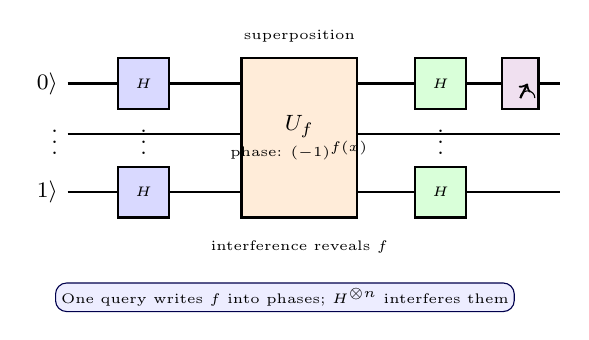
\begin{tikzpicture}[scale=0.92,font=\footnotesize]
  \draw[thick] (0,1.2)--(6.8,1.2);
  \draw[thick] (0,0.5)--(6.8,0.5);
  \draw[thick] (0,-0.3)--(6.8,-0.3);
  \node[left] at (0,1.2) {$\lvert0\rangle$};
  \node[left] at (0,0.5) {$\vdots$};
  \node[left] at (0,-0.3) {$\lvert1\rangle$};
  % H
  \draw[fill=blue!15, thick] (0.7,0.85) rectangle (1.4,1.55) node[midway, font=\tiny] {$H$};
  \node at (1.05,0.5) {$\vdots$};
  \draw[fill=blue!15, thick] (0.7,-0.65) rectangle (1.4,0.05) node[midway, font=\tiny] {$H$};
  % Oracle
  \draw[fill=orange!15, thick] (2.4,-0.65) rectangle (4.0,1.55) node[midway, align=center] {$U_f$\\{\tiny phase: $(-1)^{f(x)}$}};
  % H again
  \draw[fill=green!15, thick] (4.8,0.85) rectangle (5.5,1.55) node[midway, font=\tiny] {$H$};
  \node at (5.15,0.5) {$\vdots$};
  \draw[fill=green!15, thick] (4.8,-0.65) rectangle (5.5,0.05) node[midway, font=\tiny] {$H$};
  % meter
  \draw[fill=violet!12, thick] (6.0,0.85) rectangle (6.5,1.55);
  \draw (6.25,1.0) arc (180:0:0.1);
  \draw[->, thick] (6.25,1.0)--(6.35,1.2);
  \node[font=\tiny, fill=white, inner sep=1pt] at (3.2,1.85) {superposition};
  \node[font=\tiny, fill=white, inner sep=1pt] at (3.2,-1.05) {interference reveals $f$};
  \node[fill=blue!7, draw=blue!30!black, rounded corners, inner sep=2pt, font=\tiny] at (3.0,-1.75) {One query writes $f$ into phases; $H^{\otimes n}$ interferes them};
\end{tikzpicture}
\end{center}

\section{Deutsch and Deutsch--Jozsa}

\begin{theorem}[Deutsch 1985, $n=1$]
With one $U_f$ query, determine $f(0)\oplus f(1)$ (i.e., constant vs.\ balanced) with certainty. Classically $2$ queries are needed deterministically.
\end{theorem}
Circuit: $\lvert0\rangle\lvert1\rangle\to H^{\otimes2}\to U_f\to H$ on first qubit $\to$ measure. Outcome $0$ means constant, $1$ means balanced.

\begin{theorem}[Deutsch--Jozsa 1992]
Given promise $f$ is constant or balanced on $n$ bits, one quantum query decides which, with certainty. Any deterministic classical algorithm needs $2^{n-1}+1$ queries. Bounded-error classical needs $O(1)$ but quantum is still exact vs.\ probabilistic.
\end{theorem}
After $H^{\otimes n}U_fH^{\otimes n}$, amplitude of $\lvert0\rangle^{\otimes n}$ is $\tfrac1{2^n}\sum_x(-1)^{f(x)}$, which is $\pm1$ if constant, $0$ if balanced.

\begin{center}
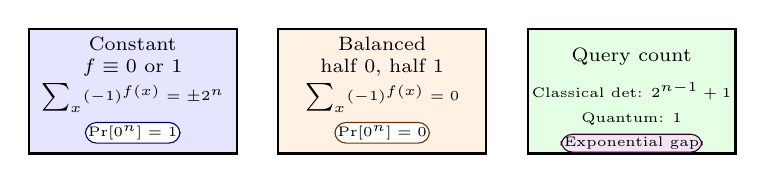
\begin{tikzpicture}[scale=0.88,font=\footnotesize]
  \fill[blue!10] (0,0) rectangle (3.0,1.8);
  \fill[orange!10] (3.6,0) rectangle (6.6,1.8);
  \fill[green!10] (7.2,0) rectangle (10.2,1.8);
  \draw[thick] (0,0) rectangle (3.0,1.8);
  \draw[thick] (3.6,0) rectangle (6.6,1.8);
  \draw[thick] (7.2,0) rectangle (10.2,1.8);
  \node[align=center, font=\scriptsize] at (1.5,1.4) {Constant\\$f\equiv0$ or $1$};
  \node[font=\tiny] at (1.5,0.8) {$\sum_x(-1)^{f(x)}=\pm2^n$};
  \node[font=\tiny, fill=white, draw=blue!40!black, rounded corners, inner sep=1pt] at (1.5,0.3) {$\Pr[0^n]=1$};
  \node[align=center, font=\scriptsize] at (5.1,1.4) {Balanced\\half $0$, half $1$};
  \node[font=\tiny] at (5.1,0.8) {$\sum_x(-1)^{f(x)}=0$};
  \node[font=\tiny, fill=white, draw=orange!40!black, rounded corners, inner sep=1pt] at (5.1,0.3) {$\Pr[0^n]=0$};
  \node[align=center, font=\scriptsize] at (8.7,1.4) {Query count};
  \node[font=\tiny] at (8.7,0.9) {Classical det: $2^{n-1}+1$};
  \node[font=\tiny] at (8.7,0.5) {Quantum: $1$};
  \node[font=\tiny, fill=violet!10, draw=violet!40!black, rounded corners, inner sep=1pt] at (8.7,0.15) {Exponential gap};
\end{tikzpicture}
\end{center}

\section{Bernstein--Vazirani}
Let $f_s(x)=s\cdot x=\bigoplus_i s_i x_i$ (parity inner product) for hidden $s\in\{0,1\}^n$.

\begin{theorem}[Bernstein--Vazirani 1993]
One quantum query recovers $s$ exactly. Classically $n$ queries are necessary. The circuit is identical to Deutsch--Jozsa; measurement yields $s$ directly.
\end{theorem}
After kickback, state is $\tfrac1{\sqrt{2^n}}\sum_x(-1)^{s\cdot x}\lvert x\rangle$, and $H^{\otimes n}$ maps it to $\lvert s\rangle$.

\begin{center}
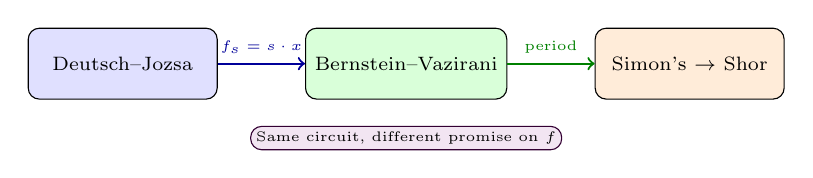
\begin{tikzpicture}[scale=0.90,font=\footnotesize]
  \node[draw, fill=blue!12, rounded corners, minimum width=2.4cm, minimum height=0.9cm, font=\scriptsize] (dj) at (0,0) {Deutsch--Jozsa};
  \node[draw, fill=green!15, rounded corners, minimum width=2.4cm, minimum height=0.9cm, font=\scriptsize] (bv) at (4.0,0) {Bernstein--Vazirani};
  \node[draw, fill=orange!15, rounded corners, minimum width=2.4cm, minimum height=0.9cm, font=\scriptsize] (sim) at (8.0,0) {Simon's $\to$ Shor};
  \draw[->, thick, blue!60!black] (dj)--(bv) node[midway, above, font=\tiny] {$f_s=s\cdot x$};
  \draw[->, thick, green!50!black] (bv)--(sim) node[midway, above, font=\tiny] {period};
  \node[font=\tiny, fill=violet!10, draw=violet!40!black, rounded corners, inner sep=2pt] at (4.0,-1.05) {Same circuit, different promise on $f$};
\end{tikzpicture}
\end{center}

These algorithms are oracular separations, not yet practical speedups, but they isolate the ingredients --- superposition, kickback, interference --- reused in Grover and Shor.

\section{Python: Simulating DJ and BV}

\begin{lstlisting}[language=Python]
import numpy as np

def hadamard_n(n):
    H = np.array([[1,1],[1,-1]])/np.sqrt(2)
    Hn = np.array([[1]], dtype=complex)
    for _ in range(n):
        Hn = np.kron(Hn, H)
    return Hn

def deutsch_jozsa(f, n):
    """Simulate DJ for f: {0..2^n-1} -> {0,1}. Return prob of |0^n>."""
    N = 2**n
    Hn = hadamard_n(n)
    # Phase oracle diag((-1)^f(x))
    phases = np.array([(-1)**f(x) for x in range(N)], dtype=complex)
    D = np.diag(phases)
    state0 = np.zeros(N, dtype=complex); state0[0]=1
    psi = Hn @ D @ Hn @ state0
    return abs(psi[0])**2  # 1 if constant, 0 if balanced

# Examples n=3
f_const = lambda x: 0
f_bal = lambda x: bin(x).count('1') % 2  # parity is balanced
print("const P(000):", deutsch_jozsa(f_const, 3))  # ~1
print("balanced P(000):", deutsch_jozsa(f_bal, 3))  # ~0
\end{lstlisting}

\begin{lstlisting}[language=Python]
# Bernstein-Vazirani: recover hidden s
def bv_circuit(s_int, n):
    N = 2**n
    Hn = hadamard_n(n)
    # f_s(x) = s.x (dot mod2)
    def f_s(x):
        return bin(s_int & x).count('1') % 2
    phases = np.array([(-1)**f_s(x) for x in range(N)], dtype=complex)
    D = np.diag(phases)
    state0 = np.zeros(N, dtype=complex); state0[0]=1
    psi = Hn @ D @ Hn @ state0
    # measurement: find index with prob 1
    probs = np.abs(psi)**2
    s_recovered = int(np.argmax(probs))
    return s_recovered, probs

for s in [0b101, 0b011, 0b110]:
    rec, _ = bv_circuit(s, 3)
    print(f"hidden {s:03b} -> recovered {rec:03b} match={rec==s}")
\end{lstlisting}

\section{Why Oracular Separations Matter}
DJ and BV do not give useful speedups on their own --- the oracles are artificial. Their value is conceptual: they prove quantum queries carry more information per call than classical bits, and they exhibit the full pipeline reused later:
\begin{enumerate}[nosep,left=10pt]
\item Prepare uniform superposition $H^{\otimes n}\lvert0\rangle$.
\item Encode $f$ into phases via $U_f$ with target $\lvert-\rangle$.
\item Interfere with $H^{\otimes n}$ to map global structure to a computational basis state.
\item Measure to read the answer with certainty.
\end{enumerate}
Grover will replace step~3 with iterative amplitude amplification; Shor will replace it with the quantum Fourier transform. The lower bounds also matter: DJ needs $2^{n-1}+1$ classical deterministic queries but only $1$ quantum query --- an exponential gap in exact query complexity. BV shows hidden linear structure $s$ is learnable in one quantum shot versus $n$ classical bits, foreshadowing learning-theoretic advantages in quantum ML.

\begin{example}[Classical simulation cost]
Simulating $H^{\otimes n}$ on $n=30$ already needs $2^{30}\approx10^9$ amplitudes --- about $16$\,GB of complex doubles. The textbook's numpy simulator handles $n\le10$ comfortably; beyond that you need a real quantum device or a tensor-network approximation. This exponential overhead is exactly what quantum hardware avoids by storing the state physically.
\end{example}


\section{Simon and Period Structure}
Simon's problem generalizes parity: $f:\{0,1\}^n\to\{0,1\}^n$ with promise $f(x)=f(y)$ iff $y=x\oplus s$. Quantumly $O(n)$ queries find $s$; classically $\Omega(2^{n/2})$ are needed (birthday bound). Simon is the template for period-finding that Shor exploits for $f(x)=a^x\bmod N$ over $\mathbb Z$, using QFT instead of Hadamards to handle periods not dividing $2^n$. The chain Deutsch $\to$ Deutsch--Jozsa $\to$ Bernstein--Vazirani $\to$ Simon $\to$ Shor traces increasingly rich hidden structure revealed by Fourier sampling.
\begin{example}[Simon $n=2$]
If $s=11$, $f$ might map $00,11\to0$, $01,10\to1$. Measuring $A\lvert0\rangle\to U_f\to H^{\otimes2}$ yields random $y$ with $y\cdot s=0$. Two independent $y$'s suffice to solve $s$ by linear algebra over $\mathbb F_2$.
\end{example}


\section{Implementation Cost and Practical Notes}
Building $U_f$ depends on $f$. For DJ/BV the constructions are cheap: BV's $s\cdot x$ needs $n$ CNOTs, DJ's arbitrary $f$ may need $O(2^n)$ gates in worst case (encoding a truth table). This is why oracular speedups do not automatically give explicit algorithmic speedups --- oracle cost must be counted. In query complexity we count queries; in time complexity we count gates to implement $U_f$. DJ's exponential gap in queries collapses if $U_f$ itself is exponentially hard.


\begin{remark}[Oracle costs]
Counting queries hides gate cost. Implementing $U_f$ for arbitrary $f$ may need $O(2^n)$ gates to encode the truth table. Thus an exponential query gap need not imply exponential time gap unless $U_f$ is efficient. For BV, $U_{f_s}$ uses $\mathrm{wt}(s)$ CNOTs, so the gap is both query and time.
\end{remark}

\begin{example}[BV oracle for $s=101$]
For $n=3$, $s=101$, $f_s(x)=x_0\oplus x_2$. Oracle uses CNOT$_{x_0\to y}$ and CNOT$_{x_2\to y}$. With $y=\lvert-\rangle$, phase kickback writes $(-1)^{x_0\oplus x_2}$. Depth $2$, width $4$, illustrating linear cost.
\end{example}

\begin{remark}[Learning perspective]
BV shows $1$ quantum vs.\ $n$ classical examples to learn $s$. This inspired quantum PAC results: discrete-log concepts are quantum-learnable with $O(n)$ examples but classically need $2^{\Omega(n)}$ under assumptions. Same Fourier primitive powers Shor.
\end{remark}

\section{Exercises}
\begin{exercise}
Work through Deutsch's algorithm step-by-step for the four functions $f:\{0,1\}\to\{0,1\}$. Show the final state before measurement is $\pm\lvert0\rangle$ if constant and $\pm\lvert1\rangle$ if balanced.
\end{exercise}
\begin{exercise}
Prove that any deterministic classical algorithm needs $2^{n-1}+1$ queries in worst case to solve Deutsch--Jozsa. What about randomized with error $\le1/3$? Show $O(1)$ samples suffice with bounded error.
\end{exercise}
\begin{exercise}
For BV with hidden $s=1011$, write the state after $U_f$ and after the final $H^{\otimes4}$. Verify it equals $\lvert s\rangle$. Trace the calculation using $H^{\otimes n}\lvert x\rangle=\tfrac1{\sqrt{2^n}}\sum_y(-1)^{x\cdot y}\lvert y\rangle$.
\end{exercise}
\begin{exercise}
Implement Simon's promise ($f(x)=f(y)$ iff $y=x\oplus s$) for $n=2$ and simulate one quantum query. What linear equations on $s$ do measurements give? How many shots are needed to find $s\neq0$?
\end{exercise}
\begin{exercise}
Show BV's oracle $U_{f_s}$ can be built with at most $n$ CNOTs from the $x$ register to the ancilla, controlled on $s_i=1$. Draw the circuit for $s=101$ and $n=3$.
\end{exercise}
